\documentclass[tikz,border=2pt]{standalone}
\usepackage{amsmath,amssymb}
\usepackage{pgfplots}
\pgfplotsset{compat=1.18}

\begin{document}
% The range is the set of values actually taken: for f(x)=x^2 on R it is [0, ∞), the shadow of
% the graph on the y-axis; negative values are in the codomain R but never reached.
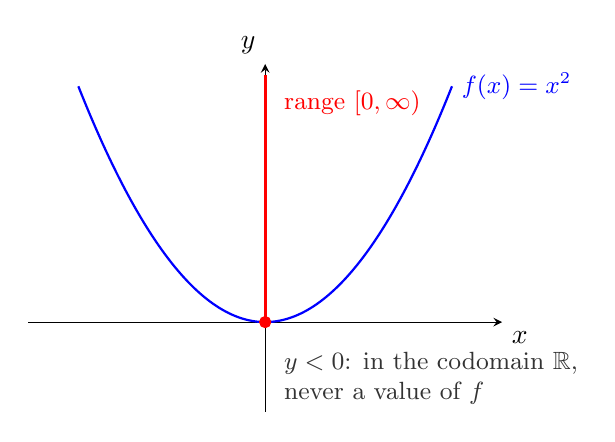
\begin{tikzpicture}
	\begin{axis}[
		axis lines=middle,
		xmin=-2.6, xmax=2.6,
		ymin=-1.6, ymax=4.6,
		xtick=\empty, ytick={0},
		xlabel={$x$}, ylabel={$y$},
		xlabel style={below right}, ylabel style={above left},
		samples=120, smooth, clip=false,
		width=7.6cm, height=6cm
		]
		\addplot[thick, blue, domain=-2.05:2.05] {x^2};
		\draw[very thick, red] (axis cs:0,0) -- (axis cs:0,4.4);
		\addplot[only marks, mark=*, red] coordinates {(0,0)};
		\node[red, anchor=west, font=\small] at (axis cs:0.1,3.9) {range $[0,\infty)$};
		\node[blue, anchor=west, font=\small] at (axis cs:2.05,4.2) {$f(x)=x^2$};
		\node[gray!40!black, anchor=west, font=\small, align=left] at (axis cs:0.1,-1.0) {$y<0$: in the codomain $\mathbb{R}$,\\ never a value of $f$};
	\end{axis}
\end{tikzpicture}
\end{document}
